\chapter{examples}
\label{chap:examples}

This chapter presents examples for some functionalities of Latex.
Of course, there is no claim to completeness, since Latex offers many different possibilities to perform additional formatting and to include other files.

First, \autoref{sec:tables_imgs} introduces ways to insert tables and images. Afterwards \autoref{sec:code} presents how to best include source code in your work.
After that, \autoref{sec:ref} is about referencing things. After that \autoref{sec:lit} briefly shows how to cite sources correctly with Latex. Other small features are introduced in \autoref{sec:other}.

The chapter concludes with an example introduction in \autoref{sec:example_intro}.

\section{images and tables}
\label{sec:tables_imgs}
\begin{figure}
	\centering
	\subfloat[Centralized control]{
		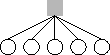
\includegraphics[width=\textwidth*2/5]{img_examples/Control_centralized.pdf}
	}
	\subfloat[Proper hierarchical control]{
		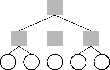
\includegraphics[width=\textwidth*2/5]{img_examples/Control_hierarchical.pdf}
	}\\
	\subfloat[Modified hierarchical control]{
		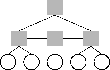
\includegraphics[width=\textwidth*2/5]{img_examples/Control_hierarchical_modified.pdf}
	}
	\subfloat[Heterarchical (distributed) control]{
		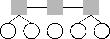
\includegraphics[width=\textwidth*2/5]{img_examples/Control_heterarchical.pdf}
	}
	\caption{Different forms of control architecture, where the control components are represented by boxes and the circles serve as controllable units, based on \cite{dilts_evolution_1991}}
	\label{Fig:ControlArch}
\end{figure}

In \autoref{Fig:ControlArch} you will see an illustration with several sub-illustrations, each of which will be included as \textit{pdf}. \textit{png} files as well as other image files can be included in the same way.

\begin{figure}
	\centering
	\def\svgwidth{\textwidth*5/11}
	\import{img_examples/}{MV.pdf_tex}
	\caption[Mandatory operating area in the MV grid, based on \cite{vde_vde-ar-n_2018-1}]{Mandatory operating area in the MV grid, based on \cite{vde_vde-ar-n_2018-1}}
	\label{Fig:MVOperating}
\end{figure}

In \autoref{Fig:MVOperating} is an example for including \textit{pdf\_tex} files, where tex-text can also be stored. Various other software, e.g., Inkscape can create such files.

\begin{table}
	\centering
	\begin{tabular}{m {3cm} | *{4}{c|} m{2.5cm}}
		Devices & \multicolumn{2}{c|}{Active power demand} & \multicolumn{2}{c|}{Reactive power demand} & Others \\
		& Increase & Decrease & Increase & Decrease & \\
		\hline
		\hline
		Inverter-based generators & + & & + & + & \\hline
		Conventional power plants & + & & + & + & Regulation of voltage level \\\hline
		Static reacitve compensating devices & & & + & + & \\\hline
		Under-load tap-changing transformers & & & & & Change of voltage level at one side \\\hline
		Energy storage systems & & + & + & + & \\hline
		Loads & & + &&&
	\end{tabular}
	\caption{Overview of devices which can support voltage regulation and their capability to increase or decrease their active or reactive power demand or to help voltage regulation in another way}
	\label{Tab:DevVolReg}
\end{table}

In \autoref{Tab:DevVolReg} you can see an example table with table caption.

\section{Source Code}
\label{sec:code}

Source code can be displayed using the \href{https://www.ctan.org/pkg/listings}{listings} package.

\begin{lstlisting}[caption=examplecode,language=python]
	def factorial(n):
	"""Program to calculate the factorial of a positive integer"""
	if n < 0:
	raise ValueError("You must enter a positive number")
	
	fact = 1
	i = 2
	while i <= n:
	fact = fact * i
	i += 1
	
	print(fact)
\end{lstlisting}

In addition to directly including the source code, a file can also be read in:
\begin{lstlisting}{name}
	\lstinputlisting[frame=single,label=examplecode,caption=anexample]{example.py}
\end{lstlisting}

\section{References}
\label{sec:ref}

There are several ways to create references.

\subsection{References to other text sections, images or tables}
First, a \textit{label} must be created to be referenced.
With \textit{ref} you can create a reference to a label with only a number, e.g. see \ref{sec:ref}. With \textit{autoref} the type label is added, e.g. see \autoref{sec:ref}. For English it is useful to use the command \textit{Cref} at the beginning of the sentence to enable proper capitalization, e.g. see \Cref{sec:ref}.

\subsection{References to the internet}
Two commands can be used to link to the Internet. With \textit{url} the URL is also displayed as text, e.g. \url{www.uol.de/des}.
With \textit{href} any text can be chosen, e.g. \href{www.uol.de/des}{Digitized energy systems}.

\section{Acronyms}
\label{sec:abbrev}
The package \textit{acronym} is used for acronyms.
The acronyms should be introduced in \textit{content/Acronyms.tex}. There are a few examples in that file. These can be included in the following way:
\begin{itemize}
	\item \textit{ac}: First mention with definition, after that only short vresion
	\item \textit{acp}: Similar to \textit{ac} but with plural
	\item \textit{acs}: Only gives the short form
\end{itemize}

The package can also be used for a list of symbols (see \textit{content/Nomenclature.tex} as example).

There is a second variant to define acronyms in \textit{content/acronymsV2.tex} which is more advanced and not compatible with overleaf. Therefore, we recommend the use of this variant only for advanced LaTeX users.

If you want to use the second option the following changes are necessary for this:
\begin{enumerate}
	\item The first option for acronyms in the \textit{main.tex} need to be commented and the second version need to be included.
	\item Instead of \textit{content/Acronyms.tex} and \textit{content/Nomenclature.tex} the other nomenclature from \textit{content/acronymsV2.tex} is now used.
	\item When compiling the PDF, \textit{\textbackslash makeindex mainThesis.nlo -s nomencl.ist -o mainThesis.nls} should be run in the terminal.
\end{enumerate}

\section{Literature}
\label{sec:lit}

In a scientific paper, assumptions must be proved. In addition, an examination of the current state of scientific research is relevant. For this purpose, appropriate sources should be cited.

For referencing sources, there is \href{https://de.wikipedia.org/wiki/BibTeX}{bibtex} in latex.
The relevant information about publications (author, title, year, etc.) is collected in the file \textit{bib/Literature.bib}. Literature management software, such as \href{https://www.citavi.com/de}{citavi} and \href{https://www.zotero.org/}{zotero}, offer an export to the format directly and also on literature websites a corresponding export of the relevant metadata is usually possible.

If you want to cite a source, it is sufficient to use the \textit{cite} command and put the identifier of the source (which can be found in the literature file at the beginning of each source) in the curly brackets.
The source will be automatically added to the bibliography.



For programming, which is often part of a thesis, mostly already existing software tools are used. If there are scientific publications about them, they should be included in the bibliography. References to the web pages of the software tools belong (including the version number and the date of retrieval) in a footnote\footnote{example: \url{https://mosaik.offis.de/}, Mosaic version: 2.5.1, accessed 2019-07-12}.

\section{sec:other}
\label{sec:other}

This section is about various small packages that may be useful.
\subsection{ToDo-Notes}
ToDo-Notes can be used to create small to-dos. The general documentation can be found at \url{https://www.ctan.org/pkg/todonotes}.
\todo[inline]{ToDos can be created \textit{inline} by specifying the additional option \textit{inline}}
\todoAsk{Normally, however, the ToDos are in the margin}
At the end of the PDF, a list of all ToDos is created.
The package is included in \textit{config/packages.tex} and all ToDos can be disabled with the \textit{disable} option.
Additional ToDo types can be created in \textit{config/commands.tex} where you can find an example.


\section{Beispieleinleitung}
\label{sec:example_intro}
Die Wettbewerbsfähigkeit energieintensiver Industrien beruht wesentlich auf einem erfolgreichen Kostenmanagement.
Die Energieausgaben bei der Herstellung sowie beim Umschlag und Transport von Gütern belasten deren Budget.
Laut Strompreisanalyse des Bundesverbandes der Energie- und Wasserwirtschaft~e.V. (2017) ist der Industriestrompreis seit dem Jahr~2000 von 6,05~ct/kWh auf 17,12~ct/kWh angestiegen (siehe Abbildung~\ref{fig:Strompr}).
Daher suchen insbesondere industrielle Betriebe sowie andere energieintensive Einrichtungen wie etwa Krankenhäuser nach Wegen, um diese Aufwendungen zu verringern.
\begin{figure}[b!]
	\centering
		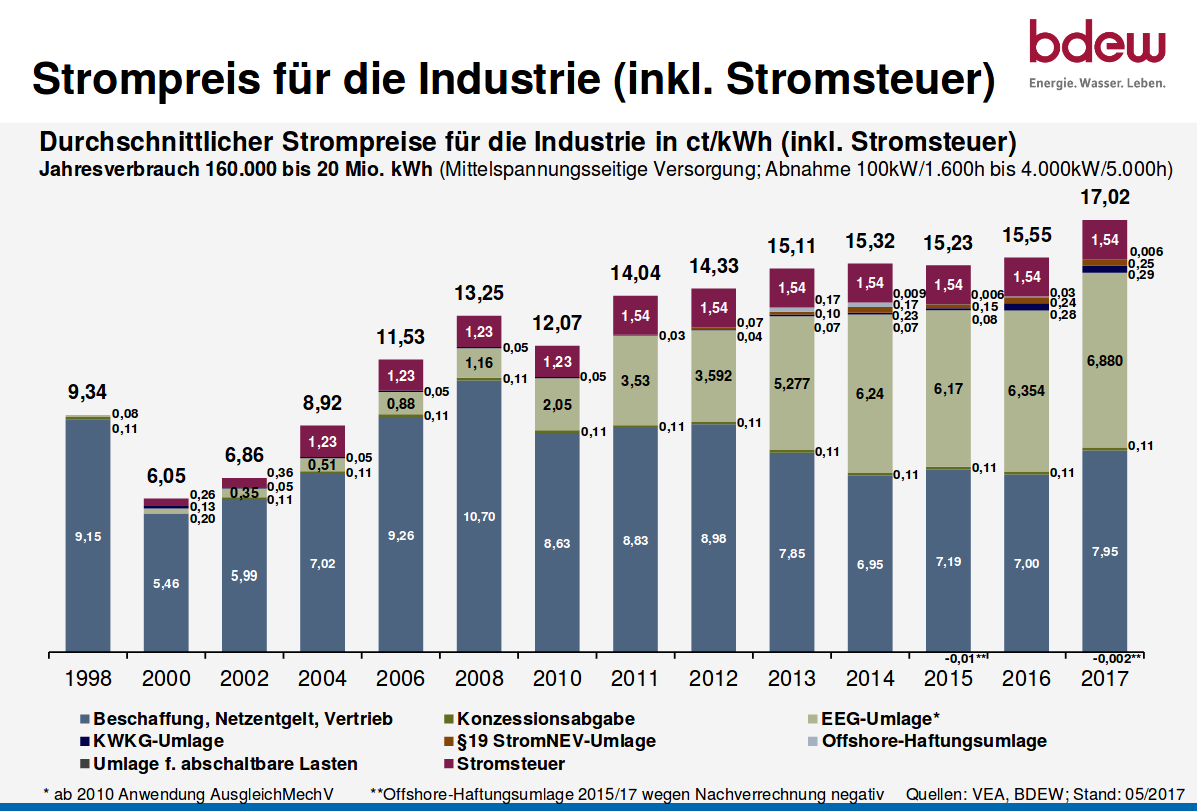
\includegraphics[width=\textwidth]{img_examples/BDEWStrompreis.png}
		\caption[Strompreisentwicklung BDEW]{Entwicklung des Strompreises für die Industrie in Deutschland von 1998 bis 2017 \cite{BDEWMai17}.		}
		\label{fig:Strompr}
\end{figure}
Beispielsweise wurden Möglichkeiten gefunden, durch eine optimierte Energiebeschaffung, durch Anwendung der \gqq{besonderen Ausgleichsregelung} \footnote{Durch die besondere Ausgleichsregelung können sich Unternehmen aus stromkosten- und handelsintensiv eingestuften Branchen von der Zahlung eines Teils der EEG-Umlage befreien lassen.}, durch Steuerbefreiung sowie durch Eigenstromerzeugung Kosten zu senken.
Verursacht durch den Netzausbau zur Aufnahme alternativer Energien steigen die Netznutzungsentgelte (NNE) seit 2011 erheblich.
\begin{figure}[tb!]
	\centering
		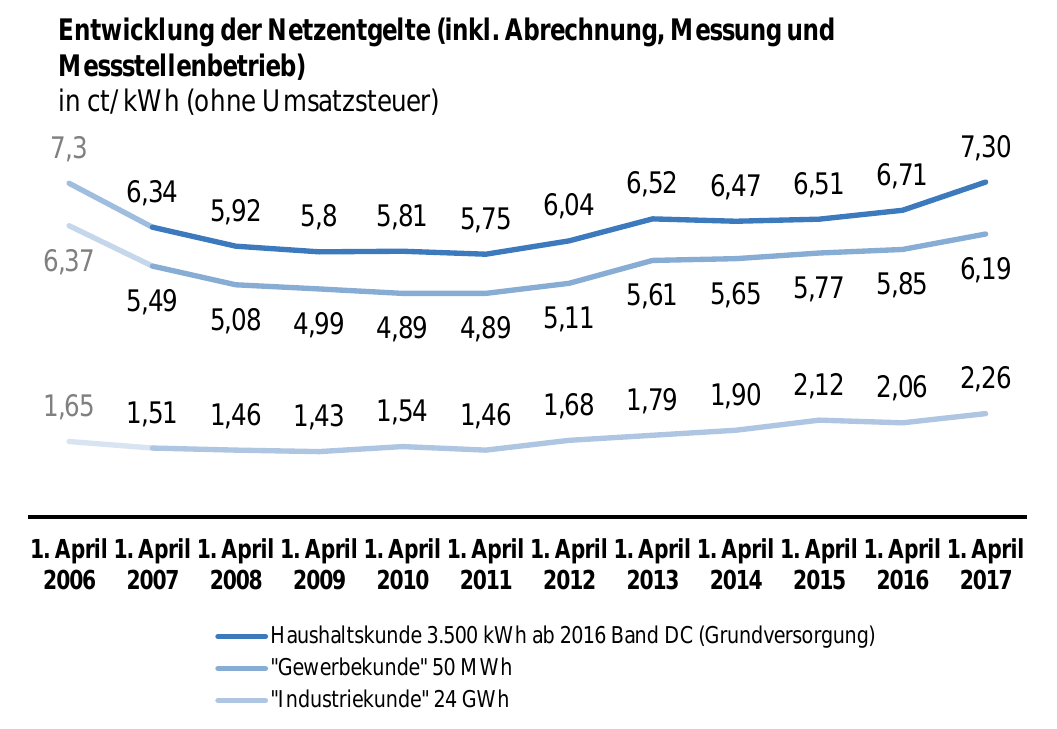
\includegraphics[width=12cm]{img_examples/BNetzANNE17.png}
		\caption[Netzentgeltentwicklung BNetzA]{Entwicklung der \aclp{NNE} in Deutschland von 2006 bis 2017 \cite{Monitor17}.
		}
		\label{fig:NNEEnt}
\end{figure}
Zwischenzeitlich waren diese seit der Einführung der Anreizregulierung im Jahr 2006 gefallen (siehe Abbildung~\ref{fig:NNEEnt}).
Daher ist es für die Industrie existenziell wichtig, Wege zur \ac{NNE}-Reduktion zu analysieren oder wenigstens ihr Potenzial für Entlastungen abzuschätzen.
Die Systematik zur Berechnung von Netzentgelten bietet für Unternehmen mit leistungsgemessen Abnahmestellen Möglichkeiten, ihre Kosten zu reduzieren.
Danach ist ein leistungsabhängiger Anteil zu entrichten, der vom maximalen Netzbezug im Abrechnungszeitraum abhängt.
Dieser wirkt sich stark auf die zu entrichtenden Beträge aus.
Aufgrund dieser Berechnungsweise des Netzentgeltes ist es wichtig, zu bestimmten Zeiten die dem Netz gegenüber an einem Anschlusspunkt auftretende Last zu reduzieren.
Anzustreben ist entweder ein verringertes allgemeines Netzentgelt oder ein niedriges individuelles Netzentgelt nach §~19~\ac{StromNEV}.
Diese unterscheiden sich dadurch, zu welchen Zeiten und in welchem Umfang Leistungsspitzen reduziert werden sollen.
%
%
\subsection{Anlass und Arbeitshypothesen der Untersuchung}
\label{Ansatz}
Durch eine Kooperation des \ac{VEA} mit dem \ac{IfES} der Leibniz Universität Hannover entstand ein Interesse, das Potenzial eines Speichereinsatzes für die deutsche Industrie genauer zu untersuchen.
Der \ac{VEA} hat dafür einen Zugriff auf sein EDV-System mit Unternehmensdatensätzen und Lastprofilen gewährt.
Im Verband sind viele energieintensive Firmen des deutschen Mittelstandes vertreten.
So kann davon ausgegangen werden, dass Ergebnisse einer solchen Untersuchung auf der Basis verfügbarer Daten repräsentativ sind für die deutsche Industrie.
Gleichzeitig steht ein vom \ac{IfES} entwickeltes Simulationsprogramm zur Verfügung, in dem Energiespeicher verschiedener Technologien einheitlich beschrieben sind.
Mithilfe der Lastgangdaten kann deren Kapazität dimensioniert und die Wirtschaftlichkeit untersucht werden.
Insgesamt waren zum Bearbeitungszeitpunkt der vorliegenden Studie vollständige Datensätze von 5360~Betrieben verfügbar.
Bei dieser gro"sen Zahl von Einzelbeispielen ist zu erwarten, dass man allgemeingültige Aussagen zur Leistungsspitzenreduktion durch Speichereinsatz machen und damit das Potenzial eines Speichereinsatzes zur \ac{NNE}-Reduzierung insgesamt beschreiben kann.
%
Im Hinblick auf diese Arbeit lassen sich zwei Hypothesen aufstellen, die auf dieser umfangreichen Datengrundlage überprüft werden sollen.
\begin{itemize}
\item Ob ein Speicher für ein Unternehmen wirtschaftlich einsetzbar ist, hängt von den Eigenschaften des Lastprofils ab.
\item Es gibt bei den Unternehmen Ausnahmefälle, in denen sich ein Speicher in sehr kurzer Zeit amortisiert.
\end{itemize}
Dies ist insofern bemerkenswert, als sich daraus folgende Konsequenz ergibt:
Durch Kenntnis der Beschaffenheit eines einzelnen Unternehmens kann direkt festgestellt werden, ob es sich lohnen würde, dort einen Speicher einzusetzen.
Ebenfalls denkbar ist, dass sich Firmen bestimmter Branchen oder auch eine Kombination bestimmter Eigenschaften für einen Speichereinsatz besser eignen als andere.
Diese Hypothesen können durch die Detailbetrachtung der 5.360 Beispielfälle überprüft werden, was erst durch das Auswerten der Daten des \ac{VEA} mit dem Werkzeug des \ac{IfES} möglich wurde.
Dabei stehen mit dem Verringern des allgemeinen Netzentgeltes durch die sog. \gqq{Spitzenlastkappung} und dem Erfüllen der Bedingungen für ein individuelles Netzentgelt verschiedene Ansätze zur \ac{NNE}-Reduktion zur Verfügung.
\begin{figure}[!tb]
	\centering
	\subfloat[Verteilung der vorliegenden Betriebe auf die angeschlossenen Netzebenen.]{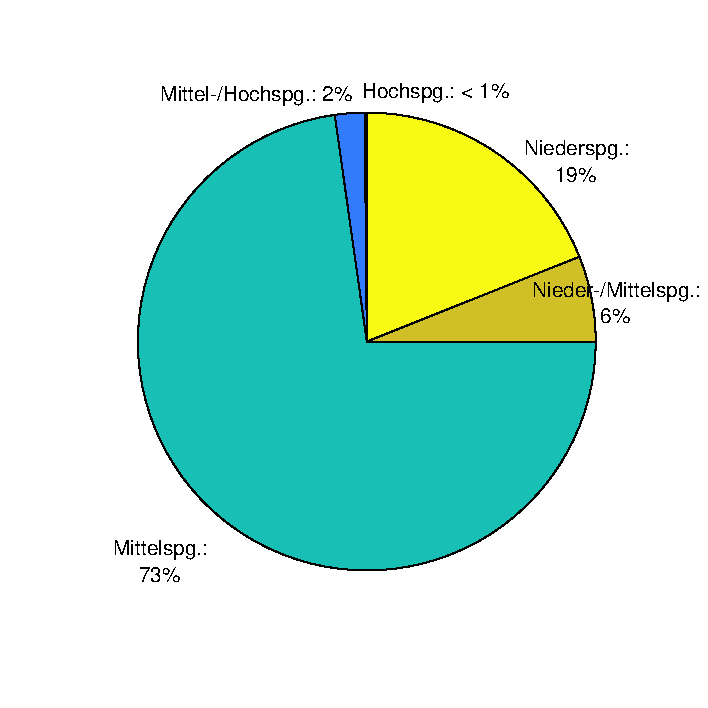
\includegraphics[width=0.4\textwidth]{img_examples/angeschNZEvert.pdf}
		%\caption[angeschlossene Netzzugangsebenen]{Über alle Datensätze betrachtet, sieht man, dass viele in der Mittel- und Niederspannung angeschlossen sind.}
		\label{fig:angeschNZEvert}} %\qquad
	\hfill
	\subfloat[Für die vorliegenden Betriebe in 2016 angewendete Leistungspreise pro Kilowatt Jahreshöchstlast.]{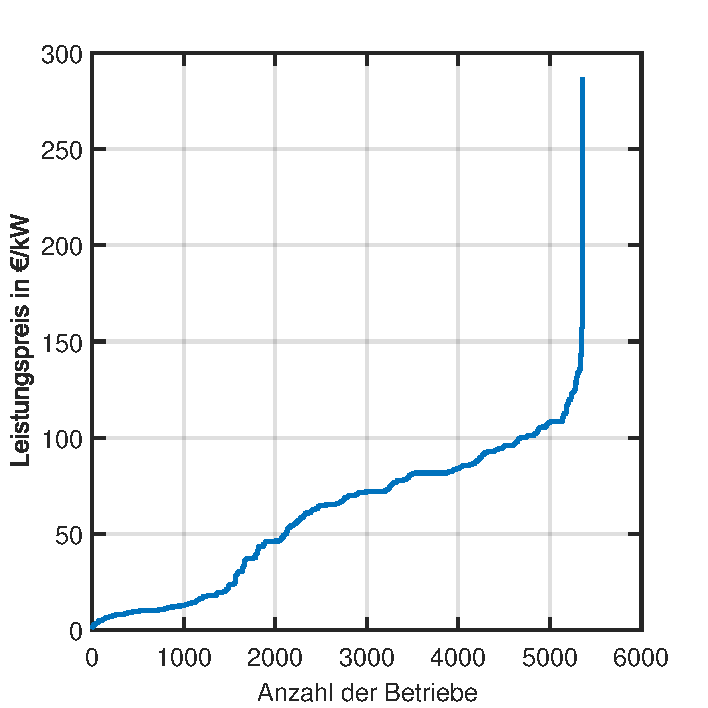
\includegraphics[width=0.4\textwidth]{img_examples/LPvert.pdf}
		%\caption[Leistungspreise über 2.500 Stunden]{Über alle Datensätze betrachtet, sieht man, dass es viele verschiedene Leistungspreise gibt.}
		\label{fig:LPvert}}
	\\
	\begin{minipage}{\textwidth}
		\subfloat[Branchenzugehörigkeit der vorliegenden Betriebe nach der Gliederung der Klassifikation der Wirtschaftszweige \cite{Branchen}.
		]{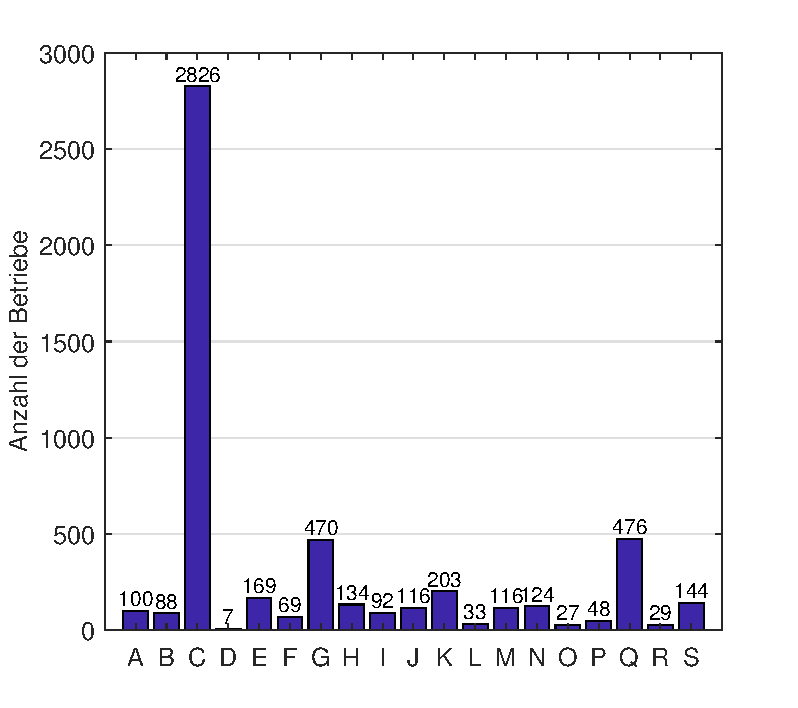
\includegraphics[width=0.5\textwidth]{img_examples/BraGrpvert.pdf}
			%\caption[Branchengruppen]{Über alle Datensätze betrachtet, sieht man, dass die meisten Firmen zum verarbeitenden Gewerbe gehören.}
			\label{fig:BraGrpvert}}
		\subfloat{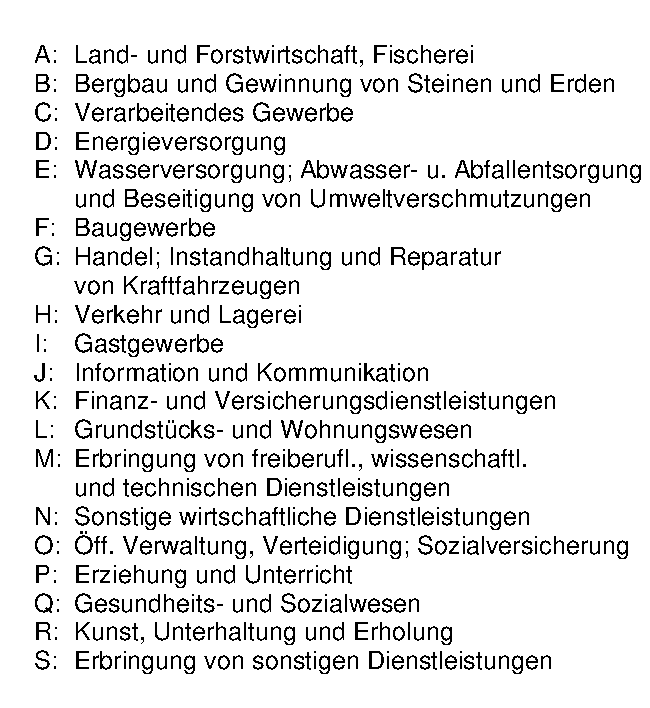
\includegraphics[width=0.45\textwidth]{img_examples/BraLabels.pdf}}
		\hfill
	\end{minipage}
	\caption[Verteilung der Betriebe auf Netzebenen, Leistungspreise und Branchen]{Beispiel für unterteilte Abbildung: Überblick über die vorliegenden Betriebe. Verteilung auf die angeschlossenen Netzebenen, die angewendeten Leistungspreise und die verschiedenen Branchen.}
	\label{fig:Verteilungen}
\end{figure}
%
Von dem Ermitteln des wirtschaftlichen Einsparpotenzials profitieren in erster Linie die Industrie und andere Unternehmen mit hohem Energiebedarf.
Sie können erfahren, unter welchen Umständen es sich für sie lohnt, in Speicher zu investieren.
Dies gilt genauso für Multiplikatoren in diesem Bereich.
Der \ac{VEA} hat gegenüber anderen Unternehmensverbänden in diesem Fall den Vorteil, dass nach Abschluss der vorgestellten Untersuchung genau bekannt ist, für welche seiner Mitglieder ein Speicher profitabel ist.
Dadurch kann er diesen gezielte Handlungsempfehlungen geben.
Die vorgestellte Untersuchung ist darüber hinaus für Akteure aus der Wissenschaft und der Speicherbranche interessant.
Unternehmen, für die ein wirtschaftlicher Speichereinsatz ermittelt wird, sind aus Sicht der Batteriehersteller potenzielle Kunden, die gezielt angesprochen werden können.
Durch Bestimmen der Kriterien, unter welchen ein Speichereinsatz für einen möglichen Kunden in Frage kommt, kann dieser leichter identifiziert und auf die Attraktivität von Speichern aufmerksam gemacht werden.
Im Rahmen einer Variation der Speicherkosten wurde beobachtet, in welchem Umfang sich die Wirtschaftlichkeit bei einer bestimmten Preisentwicklung erhöht.
Dadurch wissen Batterielieferanten, welche Kostenziele sie erreichen müssen, um neue Marktanteile zu erschlie"sen.
%
% Beispielgleichung
\begin{equation}
\label{eq:Vorl}
\Tvorl = -\tau \cdot ln \left( 1 - \frac{ 1 - \ex^{-\frac{\THLZ}{\tau}}}{\eta_{\textrm{s,cycl}}\cdot \ex^{-\frac{\THLZ}{\tau}}} \right)
\end{equation}
%
Im Folgenden wird die Systematik erklärt, wie das \ac{NNE} berechnet wird und wie es sich möglicherweise reduzieren lässt.
Außerdem wird einschlägige Literatur behandelt, die sich mit diesem und ähnlichen Themen beschäftigt.
Auf dieser Grundlage werden die Ziele dieser Arbeit definiert.
Das zweite Kapitel dient der Erklärung der verwendeten Daten, des eingesetzten Simulationsprogramms und der Wirtschaftlichkeitsberechnung.
Danach verzweigt sich die Erörterung entsprechend der genannten Ansätze.
Die zwei folgenden Kapitel behandeln eine Reduzierung der Netzentgelte mit den dafür genutzten Methoden, deren Ergebnissen und geben eine Auswertung mit anschlie"sender Diskussion.
Als erstes wird dabei die Spitzenlastkappung, der Basisfall, behandelt, und anschlie"send in Kapitel~4 die Ausnahmeregelungen nach §~19~\ac{StromNEV} erörtert.
Das letzte und fünfte Kapitel fasst die Ergebnisse zusammen und bietet einen Ausblick auf mögliche weitere Schritte.
%
\begin{table}[tb!]
	\begin{center}
			\caption{Beispiel für eine Tabelle, mit dem zugehörigen Text über der Tabelle (anders als bei Abbildungen)}
		\begin{tabular}{|c|c|}
			\hline  \thead{Information} & \thead{Wert} \\
			\hline	Betriebs-ID & 60880 \\
			\hline	Netzzugangsebene & Mittelspg. (5) \\
			\hline	Netzbetreiber &  Stadtwerke Glückstadt GmbH \\
			\hline  Arbeitspreise & \begin{tabular}{p{2cm}p{2.4cm}}\hfill <2.500~h: & \hfill 6,07~ct/kWh \\ \hfill $\geq$2.500~h: & \hfill 0,43~ct/kWh \end{tabular} \\
			\hline  Leistungspreise & \begin{tabular}{p{2cm}p{2.4cm}}\hfill <2.500~h: & \hfill 11,79~\euro/kW \\ \hfill $\geq$2.500~h: & \hfill~152,93~\euro/kW \end{tabular} \\
			\hline
		\end{tabular}
	\end{center}
	\label{tab:60880}
\end{table}